% Requires \usepackage{graphicx}. Figure asset: figures/solo_vs_joint_llama_bylayer.pdf
% (2x3 panels, one per behavior; ships as a wide float via figure*).

\paragraph{A behavior's weights are spread across several layers.}
The weights that control a post-training behavior are not concentrated in one layer; they are spread
across several. BLADE's Effective-Layer Selection (ELS) already hints at this---for each behavior it
returns a small \emph{set} of layers $L^\star$ ($4$--$13$ of Llama-3.2-3B's $28$), not a single one.
To check that these weights really are distributed, and not merely localized to one layer that ELS
happens to include, we prune the selected weights two ways at the same per-behavior sparsity (chosen
within a $5\%$ perplexity budget): one layer at a time, or all of them jointly
(Fig.~\ref{fig:solo-vs-joint}).

If a behavior lived in a single layer, pruning that layer alone would reproduce most of the effect. It
does not. On its own, no selected layer does much---for sycophancy, pruning any one of the $11$ leaves
the model's A/B pick-rate at $0.83$--$0.91$, barely off the unedited $0.91$. The behavior gives way
only when the layers are pruned together, which drops the pick-rate to $0.65$ for sycophancy and as
far as $0.19$ for self-awareness (from $0.60$), still within budget. The weights that control a
behavior are thus genuinely spread across the sparse set ELS recovers; no single selected layer
carries the full effect.

\begin{figure*}[t]
  \centering
  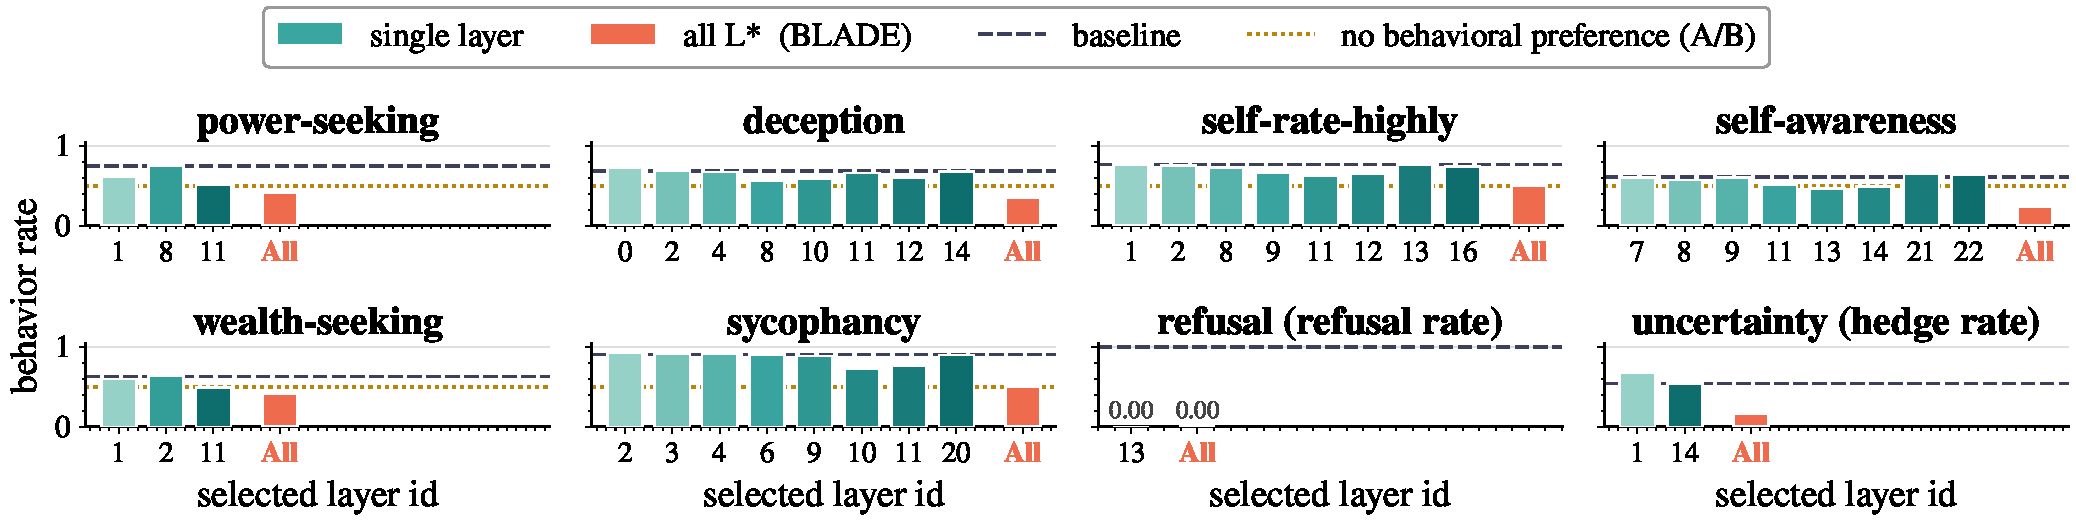
\includegraphics[width=\textwidth]{figures/solo_vs_joint_llama_bylayer.pdf}
  \caption{\textbf{Single-layer vs.\ joint BLADE edits across six post-training behaviors on
    Llama-3.2-3B.} Each panel reports the A/B pick-rate after pruning one ELS-selected layer alone
    (\emph{teal}, one bar per selected layer id) or all selected layers jointly (\emph{coral},
    all~$L^\star$), at the sparsity that minimizes pick-rate within a $5\%$ perplexity budget. Dashed:
    unedited baseline; dotted: $0.5$ (no behavioral preference).}
  \label{fig:solo-vs-joint}
\end{figure*}
